\chapter{Evaluation and Data Acquisition}
In this chapter we will provide and discuss an evaluation of our rendering approaches. For this purpose we compare our method's (peak) viewing angles with maximum reflectance for a fixed incident beam with those resulting from the grating equation at different wavelengths. But first we revisit the term diffraction grating and provide a detailed definition.

\section{Diffraction Gratings}
\label{sec:diffractiongrating}
%TODO 1. purpose
In order to evaluate the quality of our simulations, it is important to understand all underlying elements involved in the rendering process. One particular element, which we have not investigated in detail is the diffraction grating represented by our height field. Thus, in this section we will examine in detail, what a diffraction grating actually is and how it works. \\

%TODO 2. what is it
By the term $\emph{diffraction grating}$ we are referring to the surface of a flat piece of an opaque material that contains a large number of parallel, closely and evenly spaced slits$\footnote{Usually, these slits are either engraved or etched into the surface of the material.}$ or bumps. Therefore, these slits are forming a periodically packed, groove-like structure along the surface of the material. \\

% TODO 3. Purpose
A diffraction grating alters the state of an incident light beam by diffracting its component waves. According to Huygen's principle (see section $\ref{sec:huygensprincipledef}$), when an incident light beam hits the grating points on the slits, the grating will act as point light sources that emits spherical wavelets. Basically, a diffraction grating can be either transmissive (see figure $\ref{fig:idealizedtransmissivegrating}$) or reflective (see figure $\ref{fig:reflgrating}$). As light transmits through or reflects off a grating, the grooves on the grating cause different wavelengths of the light to diffract differently and thus divide the light into its component wavelengths. This also implies that the emitted wave will have a different outgoing angle with peak intensity than the incident light. In general, the closer the spacing of the slits is to the wavelength of the incident wave, the more the emitted wave will be diffracted. \\

Figure $\ref{fig:spectometer}$ illustrates what happens when a monochromatic light passes through a transmissive grating. Using a spectometer, we see that the outgoing angle of the emitted wave will be different from the incident angle. Hence, the diffracted light is composed of the sum of interfering wave components emanating from each slit in the grating.

\begin{figure}[H]
  \centering
  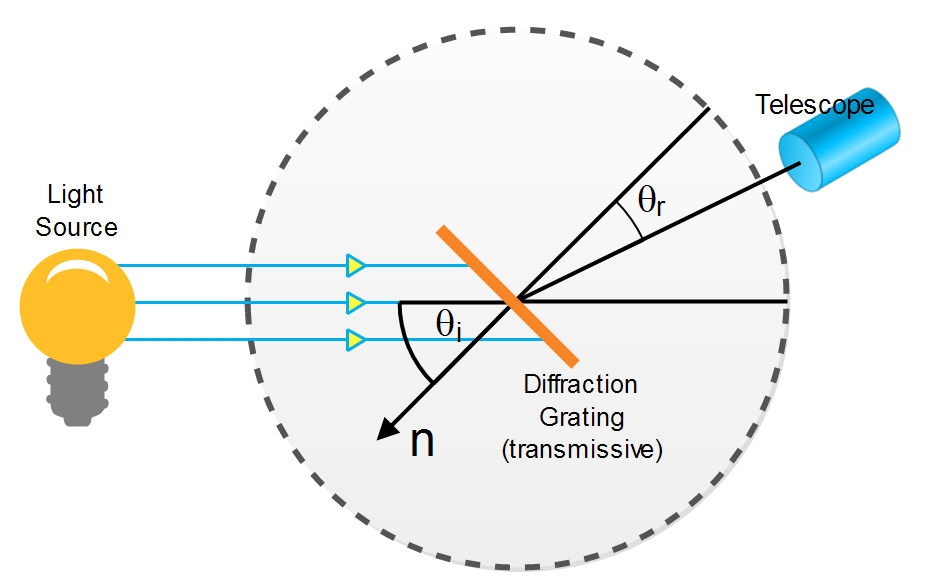
\includegraphics[scale=0.5]{evaluation/spectometer.png}
  \caption[Spectometer]{Spectometer: When a beam of monochromatic light passes through a grating placed on a spectrometer, images of the sources can be seen through the telescope at different angles.}
\label{fig:spectometer}
\end{figure}

Suppose an incident plane wavefront, composed of a monochromatic light source, is directed at a transmissive diffraction grating, parallel to its axis(i.e. its surface normal) as shown in figure $\ref{fig:lighthitsgrating}$. Let the distance between successive slits on the grating be equal to $d$. Furthermore, at a distance $L$, there is a screen parallel to the grating. Then the emitted waves will form a diffraction pattern on the screen which is the result of interference effects (constructive or destructive interference) among outgoing wavelets as shown in figure $\ref{fig:idealizedtransmissivegrating}$. 

\begin{figure}[H]
  \centering
  \subfigure[Idealized transmissive grating]{
    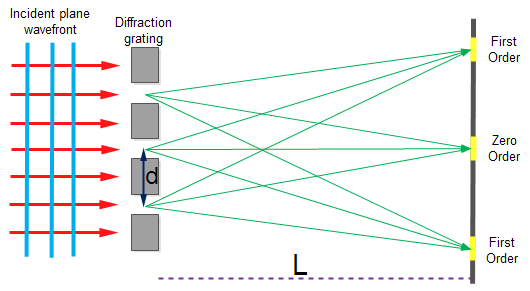
\includegraphics[scale=0.44]{evaluation/idealizeddiffgrating.png}
    \label{fig:idealizedtransmissivegrating}
  }
~  
  \subfigure[Parallel transmitted rays]{
    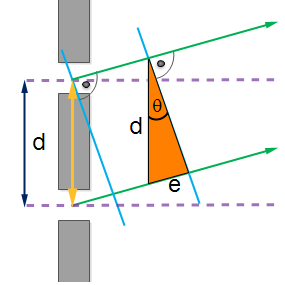
\includegraphics[scale=0.65]{evaluation/gratingsparallellines.png}
    \label{fig:gratingparallelreflectedrays}
  }

\caption[Idealized Diffraction Grating]{Light directed to parallel to grating}
\label{fig:lighthitsgrating}
\end{figure}

If the distance to the screen is much larger than the slits width, i.e. $L >> d$, then all the rays emanating from the surface and ending up at the receiver are parallel. Thus, the path difference between waves from any two adjacent slits can be derived by drawing a perpendicular line between the parallel rays. Applying simple trigonometry gives us this path difference as $e = d sin(\theta)$ as shown in figure $\ref{fig:gratingparallelreflectedrays}$. If the path difference equals one wavelength or a multiple of the wave's wavelength, the emerging, reflected waves from all slits will be in phase and a bright line will be observed at that point. Therefore, the condition for a local maxima in the interference pattern is: 

\begin{equation}
 d sin(\theta) = m \lambda 
\label{eq:simplegratingequation}
\end{equation}

where $m \in \mathds{N}_0$ is the order of diffraction and $\lambda$ is the wavelength. Because $d$ is very small for a diffraction grating, a beam of monochromatic light passing through it is split into very narrow bright fringes at large angles $\theta$ (see figure $\ref{fig:diffractionslits}$). Without the loss of generality, either for a transmissive or a reflective diffraction grating type, an analogous derivation for equation $\ref{eq:simplegratingequation}$ can be derived.

\begin{figure}[H]
  \centering
  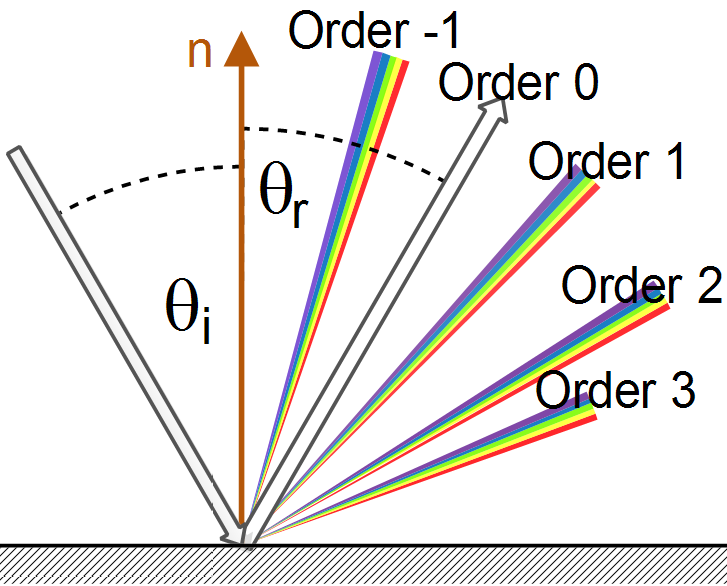
\includegraphics[scale=0.55]{evaluation/GratingSurface.png}
  \caption[Different Diffraction Orders]{Illustration of different diffraction orders when light is diffracted on a reflective diffraction grating. An incident beam of light hits a surface at an angle $\theta_i$ w.r.t. the surface normal $n$. The angle $\theta_r$ denotes the angle of the reflected beam (zero order).}
\label{fig:gratingdiffractionorders}
\end{figure}

When a beam of white light is directed at a diffraction grating along its axis, instead of a monochromatic bright fringe, a set of colored spectra are observed on both sides of the central white band. Figure $\ref{fig:diffractionslits}$ illustrates this for different number of slits on a diffraction grating. 

\begin{figure}[H]
  \centering
  \subfigure[one slit]{
    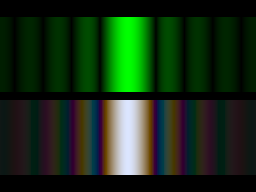
\includegraphics[scale=0.19]{evaluation/slits/spalt1.png}
    \label{fig:diffractionSlits1}
  }
  \subfigure[seven slits]{
    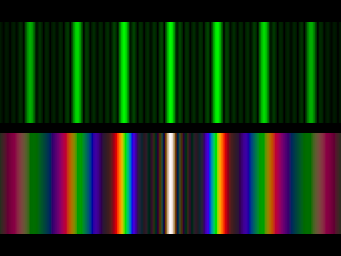
\includegraphics[scale=0.19]{evaluation/slits/spalt07.png}
    \label{fig:diffractionSlits7}
  }
  
\caption[N Slit Diffraction Grating Pattern]{Difference of diffraction pattern$\footnotemark$ between a monochromatic (top) and a white (bottom) light spectra for different number of slits.}
\label{fig:diffractionslits}
\end{figure}
\footnotetext{These images have been taken from \texttt{http://www.itp.uni-hannover.de/\textasciitilde zawischa/ITP/multibeam.html}}

Since the reflection angle $\theta_r$ for a maxima increases with wavelength $\lambda$, red light, which has the longest wavelength, is diffracted through the largest angle. Similarly violet light has the shortest wavelength and is therefore diffracted the least. Thus, white light is split into its component colors from violet to red light. The spectrum is repeated in the different orders of diffraction, emphasizing certain colors differently, depending on their order of diffraction like shown in figure $\ref{fig:gratingdiffractionorders}$. Note that only the zero order spectrum is pure white. Figure $\ref{fig:nslitdiffractionintensity}$ shows the relative intensity resulting when a beam of light hits a diffraction grating with different number of slits. From the graph we recognise that the more slits a grating has, the sharper more slopes the function of intensity gets. This is similar like saying that, the more periods a grating has, the sharper the diffracted color spectrum gets like shown in figure $\ref{fig:diffractionslits}$. 

\begin{figure}[H]
  \centering
  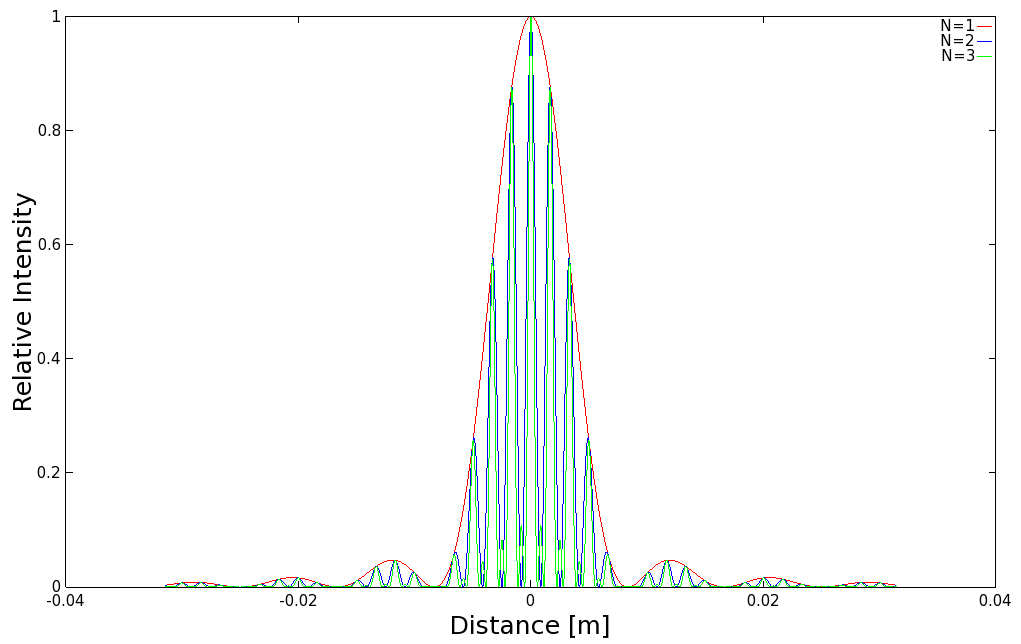
\includegraphics[scale=0.6]{evaluation/relativeintensivity.png}
  \caption[Intensity Plots for Different Number of Slits]{Relative intensities of a diffracted beam of light with wavelength $\lambda=500nm$ on a grating for different number of slits $N$. A slit width of 30 microns and a slit separation of 0.15 mm was used. The viewer is 0.5m away from the grating.}
  \label{fig:nslitdiffractionintensity}
\end{figure}

\section{Data Acquisition}
Our goal is to perform physically accurate simulations of diffraction effects due to natural gratings. As for every simulation, its outcome highly depends on the input data and thus we also require measurements$\footnote{All measured data has been provided by the Laboratory of Artificial and Natural Evolition at Genava - Website:\texttt{www.lanevol.org}}$ of real natural gratings. For that purpose, samples of skin sheds of Xenopeltis and Elaphe snake species were fixed on a glass plate. Then, by using an Atomic Force Microscope (AFM), their surface topography was measured and digitally stored$\footnote{Note these measured height fields can be visualized using grayscale images, indicating their relative depth.}$. In general, an AFM is a microscope that uses a tiny probe mounted on a cantilever to scan the surface of an object. The probe is extremely close to the surface, but does not touch it. As the probe traverses the surface, attractive and repulsive forces arising between it and the atoms on the surface inducing forces on the probe that bends the cantilever. The amount of bending is measured and recorded, providing a depth-map of the atoms on the surface. An atomic force microscope is a very high-resolution probe scanner with its demonstrated resolution on the order of a fraction of a nanometer, which is more than 1000 times better than the optical diffraction limit. The resolution of any optical system is limitted by the optical diffraction limit due to the effect of diffraction. Thus, no matter how well a lense of an optical system is corrected, its resolution is fundamentally limited by this optical barrier.

\section{Verifications}
\label{sec:approachesverifications}
\begin{figure}[H]
  \centering
  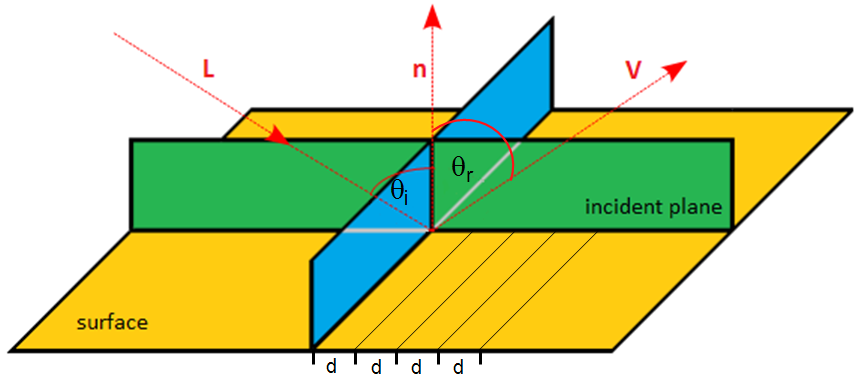
\includegraphics[scale=0.65]{evaluation/evalsetup2.png}
  \caption[Experimental Setup]{Experimental setup for evaluation: A light beam with direction $L$ hits the surface, representing a grating pattern with periodicity $d$, at the incident plane$\footnotemark$ relative to the surface normal $n$ at angle $\theta_i$ and emerges at an angle $\theta_r$ with viewing direction $V$.}
  \label{fig:experimentalsetup}
\end{figure}
\footnotetext{Remember that in general a direction vector is determined by two angles. In our evaluation setup one angle is initially fixed. Thus, regardless what value we choose for our free angle parameter the incident light will always be parallel to a so called incident plane (green plane shown in figure $\ref{fig:experimentalsetup}$.}

The physical reliability of our BRDF models has been verified by applying it to a height field for a synthetic blazed grating. Figure $\ref{fig:experimentalsetup}$ illustrates the geometrical setup for our evaluation approach: A monochromatic beam of light with wavelength $\lambda$ hits a surface with periodicity $d$ at an angle $\theta_i$ relative to the normal $n$ along its incident plane. The beam emerges from the surface at the angle $\theta_r$ with certain intensity as predicted by our model. Note that actually two angles are necessary in order to define a direction vector, using spherical coordinates. However, in our evaluation we fixed the azimuthal angle of these directional vectors (Further information can be found in section $\ref{sec:evalprecomp}$). \\

In our evaluation we compare the local peak angles predicted by our model with those resulting from the grating equation $\ref{eq:gratingeq}$. The grating equation models the relationship between the grating spacing, the incident light angle and the angle for a local maxima for the diffracted light beam. 

\begin{figure}[H]
  \centering
  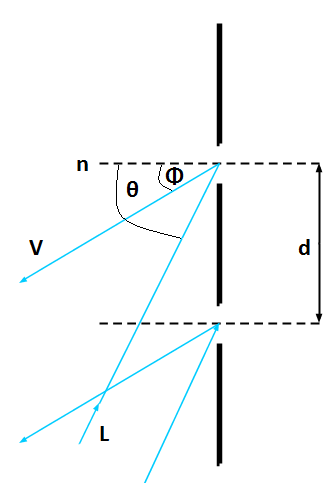
\includegraphics[scale=0.45]{evaluation/reflgrating.png}
  \caption[Reflective Grating]{Reflecting grating: When the incident light direction is not parallel to its axis at the grating there is another $sin(\phi)$ involved. See also the grating equation $\ref{eq:gratingeq}$.}
  \label{fig:reflgrating}
\end{figure}
\noindent
Figure $\ref{fig:reflgrating}$ shows that if the incident light is not along the axis of the diffraction gratings then it effects the optical path differences. The angles with locally maximum intensity is given by the grating equation derived from the equation $\ref{eq:simplegratingequation}$ following figure $\ref{fig:reflgrating}$: 

\begin{equation}
  sin(\theta_i) = sin(\theta_r) + \frac{m \lambda}{d}
\label{eq:gratingeq}
\end{equation}

In our evaluation we are interested in the first order diffraction, i.e. $m=1$. We further assume that the incident light direction $L$ is given. In contrast the direction of the reflected wave $V$ is a free parameter. \\

In Mathematics, a three dimensional direction vector is fully defined by two angles, i.e. it can be represented by spherical coordinates. Hence, $\theta_i$, is a given constant whereas $\theta_r$ is a free parameter for our evaluation simulation. Therefore, we are going to compare the maxima or the peak viewing angles corresponding to each wavelength using data produced from our method against the maxima resulting by the grating equation $\ref{eq:gratingeq}$.

\subsection{Numerical Comparisons}
\label{sec:evalprecomp}
In this section we explain how we evaluated the quality of our BRDF models. For a fixed incident light direction we want to compare the peak viewing angles with maximum reflectance for our method with those resulting from the grating equation for different wavelengths. For this purpose we realized the BRDF models corresponding to different gratings for each of our shading approaches, FLSS, NMM and PQ, in Java. By fixing the azimuth angle$\footnote{Each direction vector in space can be expressed by spherical coordinates. Then, such a unit vector is defined by a pair of two angles, the inclination and the azimuth angle. For further information, please have a look at appendix $\ref{sec:sphericalcoordinates}$}$ of the incident light $L$- and viewing direction $V$, we reduced the degrees of freedom due to these directions, during our evaluation. Thus, any BRDF is then defined by a function that expects as input arguments a wavelength $\lambda$, the inclination angle of the incident light $\theta_i$ - and the viewing direction $\theta_r$. The return value of such a function, denoted by $BRDF(\lambda, \theta_i, \theta_r)$, is the intensity value of the corresponding BRDF at these given input arguments. \\

For further details how we evaluated our BRDF in Java and how we generated the corresponding evaluation plots, please refer the appendix chapter $\ref{chap:appendixevaldatagen}$.

\subsection{Virtual Testbench}
\label{sec:virtualtestbench}
\begin{figure}[H]
  \centering
  \subfigure[Blazed Grating]{
    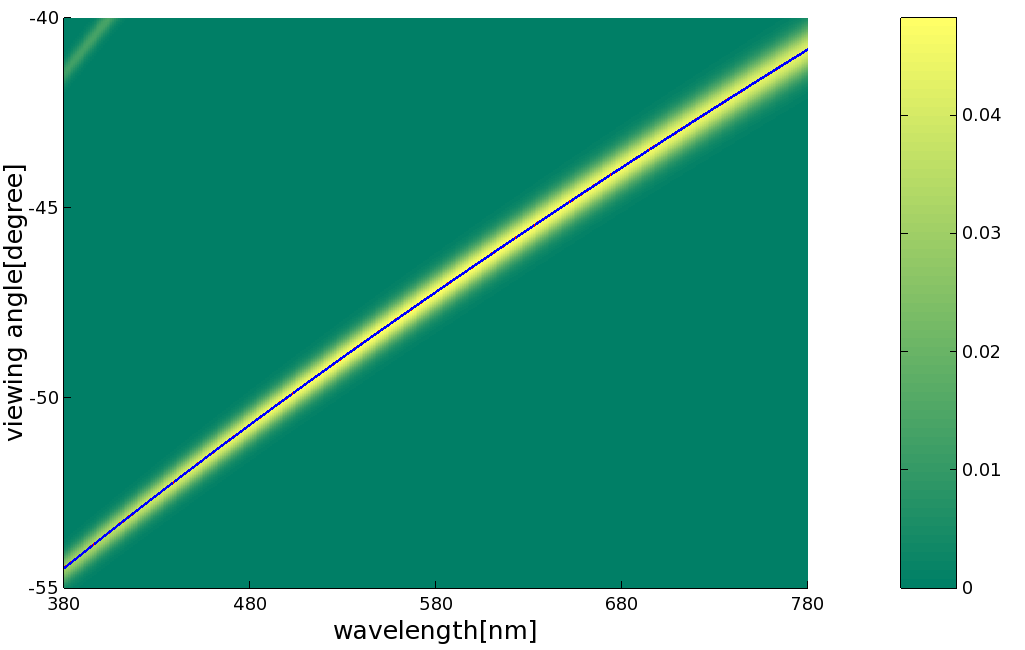
\includegraphics[scale=0.26]{evaluation/verification/flss_blazed.png}
    \label{fig:blazeval}
  }
~
  \subfigure[Xenopeltis Grating]{
    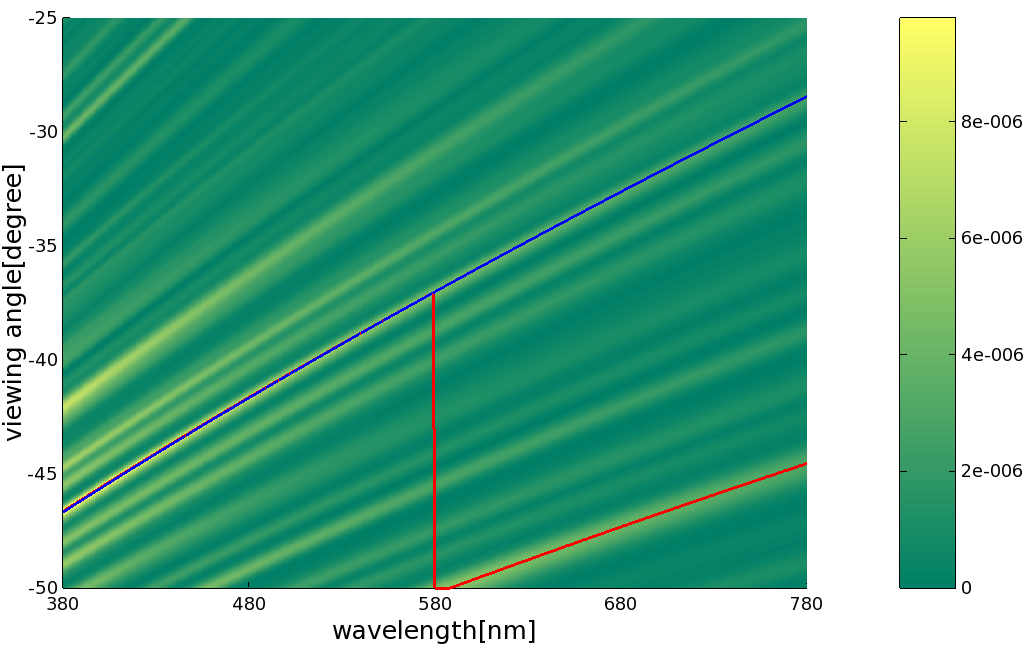
\includegraphics[scale=0.26]{evaluation/verification/flss_xeno.png}
    \label{fig:xenopeltiseval}
  }
  
\subfigure[Elaphe Grating]{
  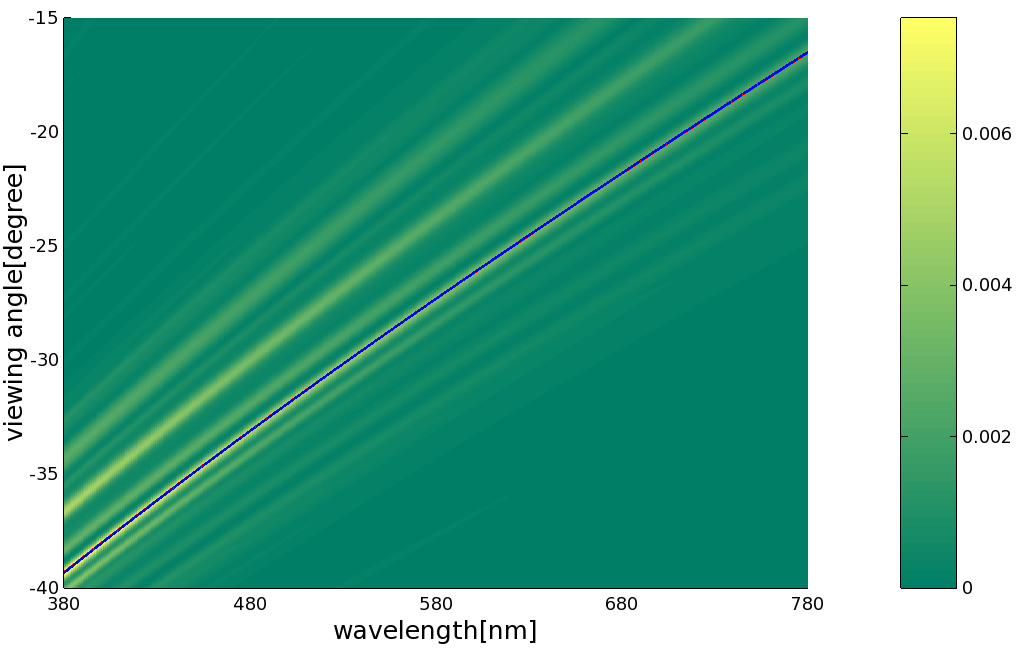
\includegraphics[scale=0.5]{evaluation/verification/flss_elaphe.png}
  \label{fig:elapheeval}
}

\caption[Validation of FLSS Approach applied on our Gratings]{Reflectance obtained by using the FLSS approach described in algorithm $\ref{alg:fragmentshaderall}$.}
\label{fig:evaluationdiffshaderalllambda}
\end{figure}

In this section we discuss the quality of our BRDF models applied to different surface structures. For that purpose we compare the resulting relative reflectance computed as described in section $\ref{sec:evalprecomp}$ for each of our BRDF models to the idealized grating equation $\ref{eq:gratingeq}$. 

\begin{table}[H]
\centering
\begin{tabular}{|l|c|c|c|c|c|c|}
\hline
\multicolumn{1}{|c|}{\multirow{3}{*}{\begin{tabular}[c]{@{}c@{}}Measuring\\ periodicity $d$\\ in [nm]\end{tabular}}} & \multicolumn{6}{c|}{Method}                                                    \\ \cline{2-7} 
\multicolumn{1}{|c|}{}                                                                                           & \multicolumn{2}{c|}{FLSS} & \multicolumn{2}{c|}{NMM} & \multicolumn{2}{c|}{PQ} \\ \cline{2-7} 
\multicolumn{1}{|c|}{}                                                                                           & mean        & variance    & mean        & variance   & mean       & variance   \\ \hline
Blazed Grating                                                                                                   & 2499.997    & 0.377       & 2499.997    & 0.377      & 2491.861   & 248.044    \\ \hline
Elpahe Grading                                                                                                   & 1144.262    & 0.401       & 1144.179    & 0.677      & 1052.308   & 49.678     \\ \hline
Xenopeltis Grating                                                                                               & 1552.27     & 0.45        & -           & -          & -          & -          \\ \hline
\end{tabular}
\caption[Estimated Grating Spacings]{Statistics of periodicity $d$ of our used gratings $\ref{fig:gratingpatches}$ estimated by using the grating equation $\ref{eq:gratingeq}$.}
\label{tab:gratingsmeanvariance}
\end{table}

Figure $\ref{fig:evaluationdiffshaderalllambda}$ shows the reflectance graphs (BRDF response) resulting from the FLSS approach over the \emph{wavelength-spectrum-reflected-light-angle} grid $\left( \Lambda, \Theta \right)$ (according to the equations $\ref{eq:lambdaspacesetup}$ and $\ref{eq:thetaspacesetup}$ as described in the appendix chapter $\ref{chap:appendixevaldatagen}$) as described in algorithm $\ref{alg:fragmentshaderall}$. This evaluation was applied to an idealized periodic structure, namely to the Blaze- $\ref{fig:blazeval}$ and to two natural gratings, the Elaphe- $\ref{fig:elapheeval}$ and Xenopeltis grating $\ref{fig:xenopeltiseval}$. For all our evaluation plots, we used an illumination angle of $\theta_i$ equal to $75\degree$. \\

Note that higher response values are plotted in yellow and lower values in green. For each of the graphs we determine the viewing angles with peak reflectance for each wavelength and then plot these peak viewing angles versus corresponding wavelengths as solid red curves. The blue curve represents diffraction angles for an idealized periodic structure with a certain periodicity $d$ according to the grating equation $\ref{eq:gratingeq}$. In the following we explain how the value $d$ is computed. \\

By rearranging the terms of the grating equation defined in equation $\ref{eq:gratingeq}$ and using the peek reflectance angle $\alpha_{r_k}$ derived like in algorithm $\ref{alg:evalmatlab}$ using the matrix $R$ of equation $\ref{eq:responsematrix}$, we can compute a periodicity vale $d_k$ for any wavelength $\lambda_k$.  
\begin{equation}
  d_k = \frac{\lambda}{sin(\alpha_{r_k}) + sin(\theta_i)}
\end{equation}

By computing the mean value of these $d_k$ values for all $\lambda$ in $\Lambda$ we can compute an estimated periodicity value $d$. We estimated these periodicity values for every grating structure and every method we are using. Thes corresponding periodicity values are tabulated in table $\ref{tab:gratingsmeanvariance}$. \\

The red and blue curve are closely overlapping in the figure $\ref{fig:blazeval}$ (for a blazed grating) and $\ref{fig:elapheeval}$ (for an Elaphe grating). For Blaze and Elaphe there is only diffraction along one direction perceivable. Since the Blazed grating is synthetic we use its exact periodicity to plot the blue curve instead of estimating it. For Xenopeltis it is interesting to see that the red curve for the peak viewing angle toggles between two ridges corresponding to two different periodicities. This happens because there are multiple subregions of the nanostructure with slightly different orientations and periodicity. Each subregion carves out a different yellowish ridge. Depending on the viewing angle, the reflectance of such a subregion can be higher than others. \\

Figure $\ref{fig:evaluationdiffshadernminmax}$ shows the evaluation plots for the NMM approach applied to the Blazed- (see figure $\ref{fig:elapheneval}$) and the Elaphe-grating (see figure $\ref{fig:elapheneval}$). The NMM approach is an optimization of the FLSS approach and is discussed in section $\ref{sec:nmmapproach}$. The response curve of each plotted NMM approach graph closely matches the corresponding grating equation curve. Furthermore, the evaluation graphs of the NMM approach look similar to the corresponding evaluation plots of the FLSS approach shown in figure $\ref{fig:evaluationdiffshaderalllambda}$. Thus, this confirms that the NMM optimization works well.

\begin{figure}[H]
  \centering
  \subfigure[Blaze grating]{
    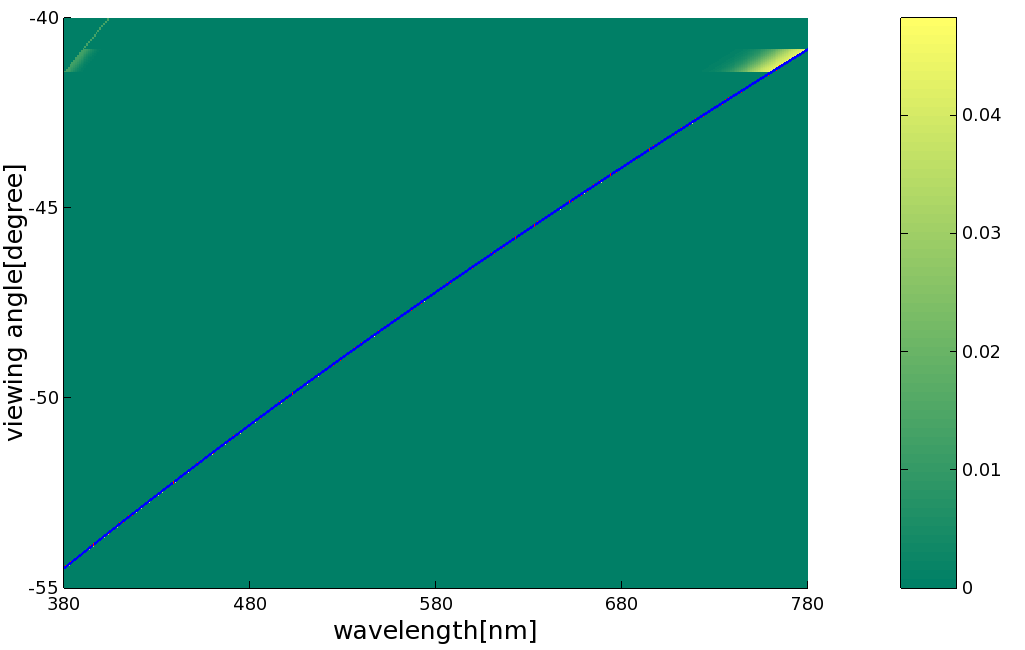
\includegraphics[scale=0.26]{evaluation/verification/nmm_blazed.png}
    \label{fig:blazneval}
  }
~
  \subfigure[Elaphe grating]{
    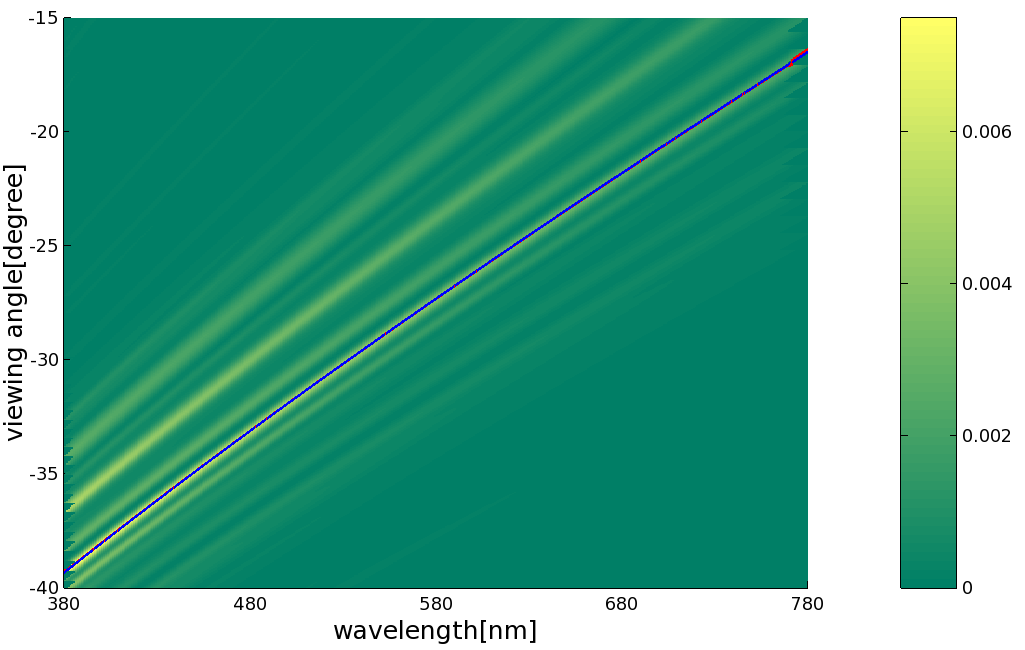
\includegraphics[scale=0.26]{evaluation/verification/nmm_elaphe.png}
    \label{fig:elapheneval}
  }
\caption[Validation of NMM Approach applied on our Gratings]{Reflectance obtained using NMM optimization apporach.}
\label{fig:evaluationdiffshadernminmax}
\end{figure}

Last, let us consider the evaluation graphs in figure $\ref{fig:evaluationdiffshaderpq}$ for the PQ approach described in algorithm $\ref{alg:sincinterpolation}$. The PQ approach assumes the given grating being periodically distributed on the surface of a shape. For this approach we have plotted evaluation graphs of the Blaze- (See figure $\ref{fig:blazepqeval}$) and Elaphe grating (See figure $\ref{fig:elaphepqeval}$). The response curves of both PQ evaluation graphs exhibit some similarities, but also some differences, compared to their corresponding grating equation curves. We could say that the response curve of the blaze grating is weakly oscillating around the grating equation curve (blue), but basically following it even with some outliers. The response curve of the Elpahe grating is not following its corresponding first order grating equation curve well. This could be due to the PQ's assumption that a given height field has to be periodically distributed along the surface. But in general, for natural gratings, this assumption usually does not hold true. Nevertheless, the red curve fits one of the response curves. We conclude that the PQ approach produces inaccurate results compared to the FLSS approach. Thus, the PQ approach is sub-optimal and unusable in practice.

\begin{figure}[H]
  \centering
  \subfigure[Blaze grating]{
    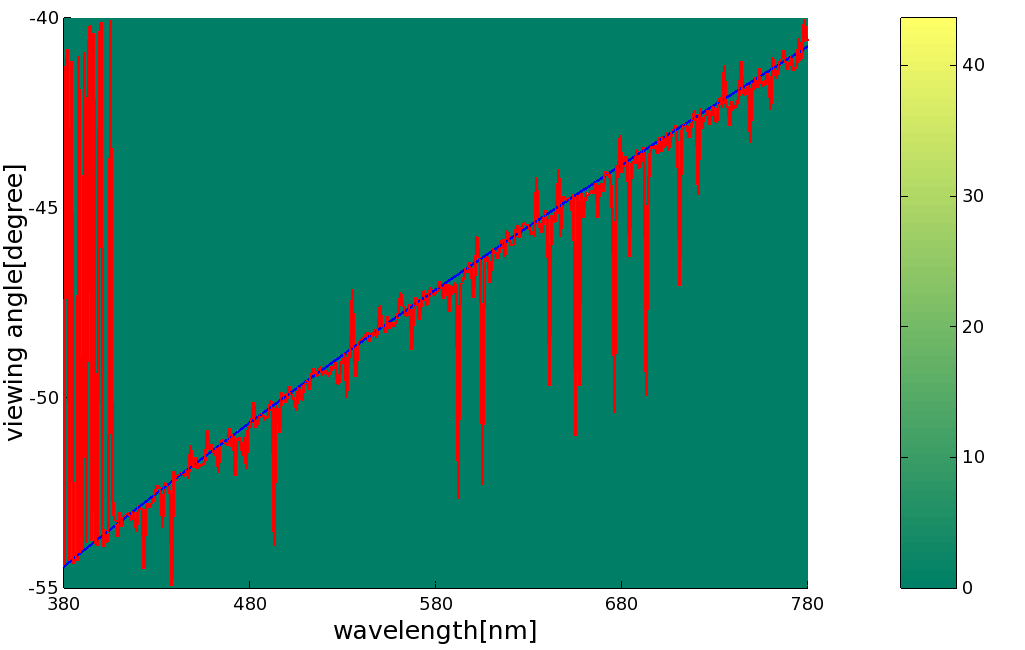
\includegraphics[scale=0.26]{evaluation/verification/pq_blazed.png}
    \label{fig:blazepqeval}
  }
~
  \subfigure[Elaphe grating]{
    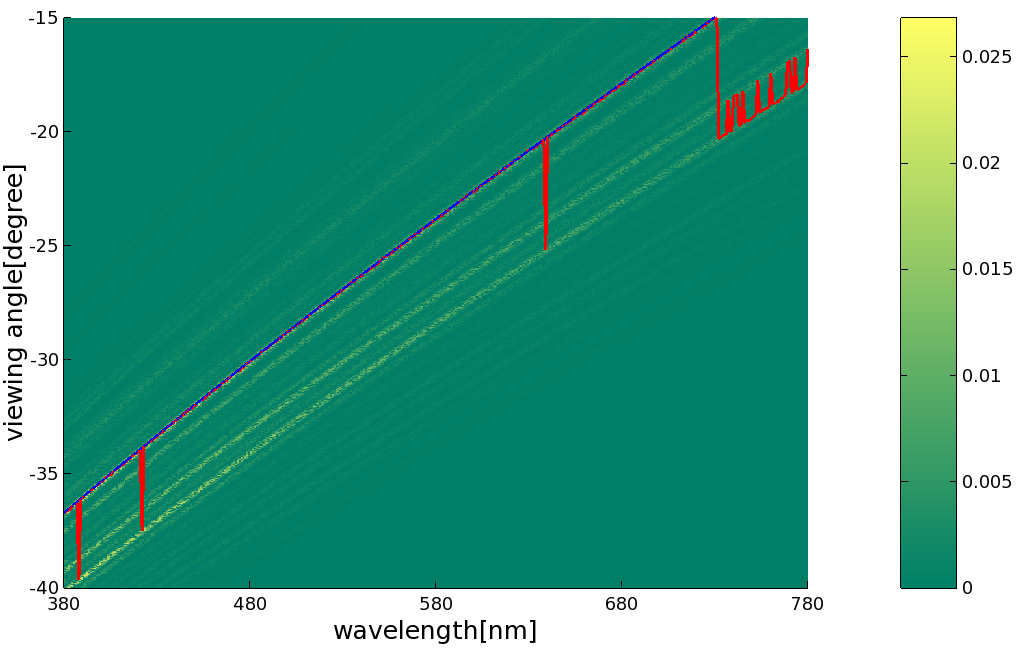
\includegraphics[scale=0.26]{evaluation/verification/pq_elaphe.png}
    \label{fig:elaphepqeval}
  }
\caption[Validation of PQ Approach applied on our Gratings]{Reflectance obtained using PQ optimization approach.}
\label{fig:evaluationdiffshaderpq}
\end{figure}
